%checked by Mark May 9th 2019
\section{Proximity and Visual Fidelity}
\label{sec:contacts:visualising}

As part of the Social AR Continuum, representing social contacts of self and others is one of the main dimensions. This section explores representing social contacts in the form of avatars in AR. 

One of the issues with representing contacts from social networks in AR is how to differentiate between the contacts. This section explores how visual and spatial cues based on social relationships can be used to represent contacts in social AR applications, making it easier to distinguish between them \cite{Nassani2017b}. This section explores how to visualise social relationships in mobile AR environments using proximity and visual fidelity filters. A focus group was organised to explore different options for representing social contacts in a mobile AR application. Also, a user study was conducted to test a head-worn AR prototype using proximity and visual fidelity filters. 

Visualising of social contacts traditionally has been represented as a list of names and a profile photo, which can be found in popular social networking mobile and web apps such as Facebook\footnote{https://www.facebook.com/}, Whatsapp\footnote{https://www.whatsapp.com/}, LinkedIn\footnote{https://www.whatsapp.com/} and others. In Google\texttt{+} \footnote{https://en.wikipedia.org/wiki/Google\%2B}, social contacts are represented as a graph of circles interconnected based on common interest and how people know each other. In Snapchat\footnote{https://www.snapchat.com/}, social contacts are also represented as a list in addition to a map feature where it shows friends as avatars overlaid on a map based on their geographical location. The avatars in Snapchat are created using Bitmoji\footnote{https://www.bitmoji.com/}, which allows the user to customise the appearance of their avatar that can be used to express predefined gestures representing emotions and interactions. Snapchat also uses these Bitmoji in sharing an AR scene where the avatar is overlaid on the camera view of a handheld device. 

\begin{figure}[h]
    \centering
    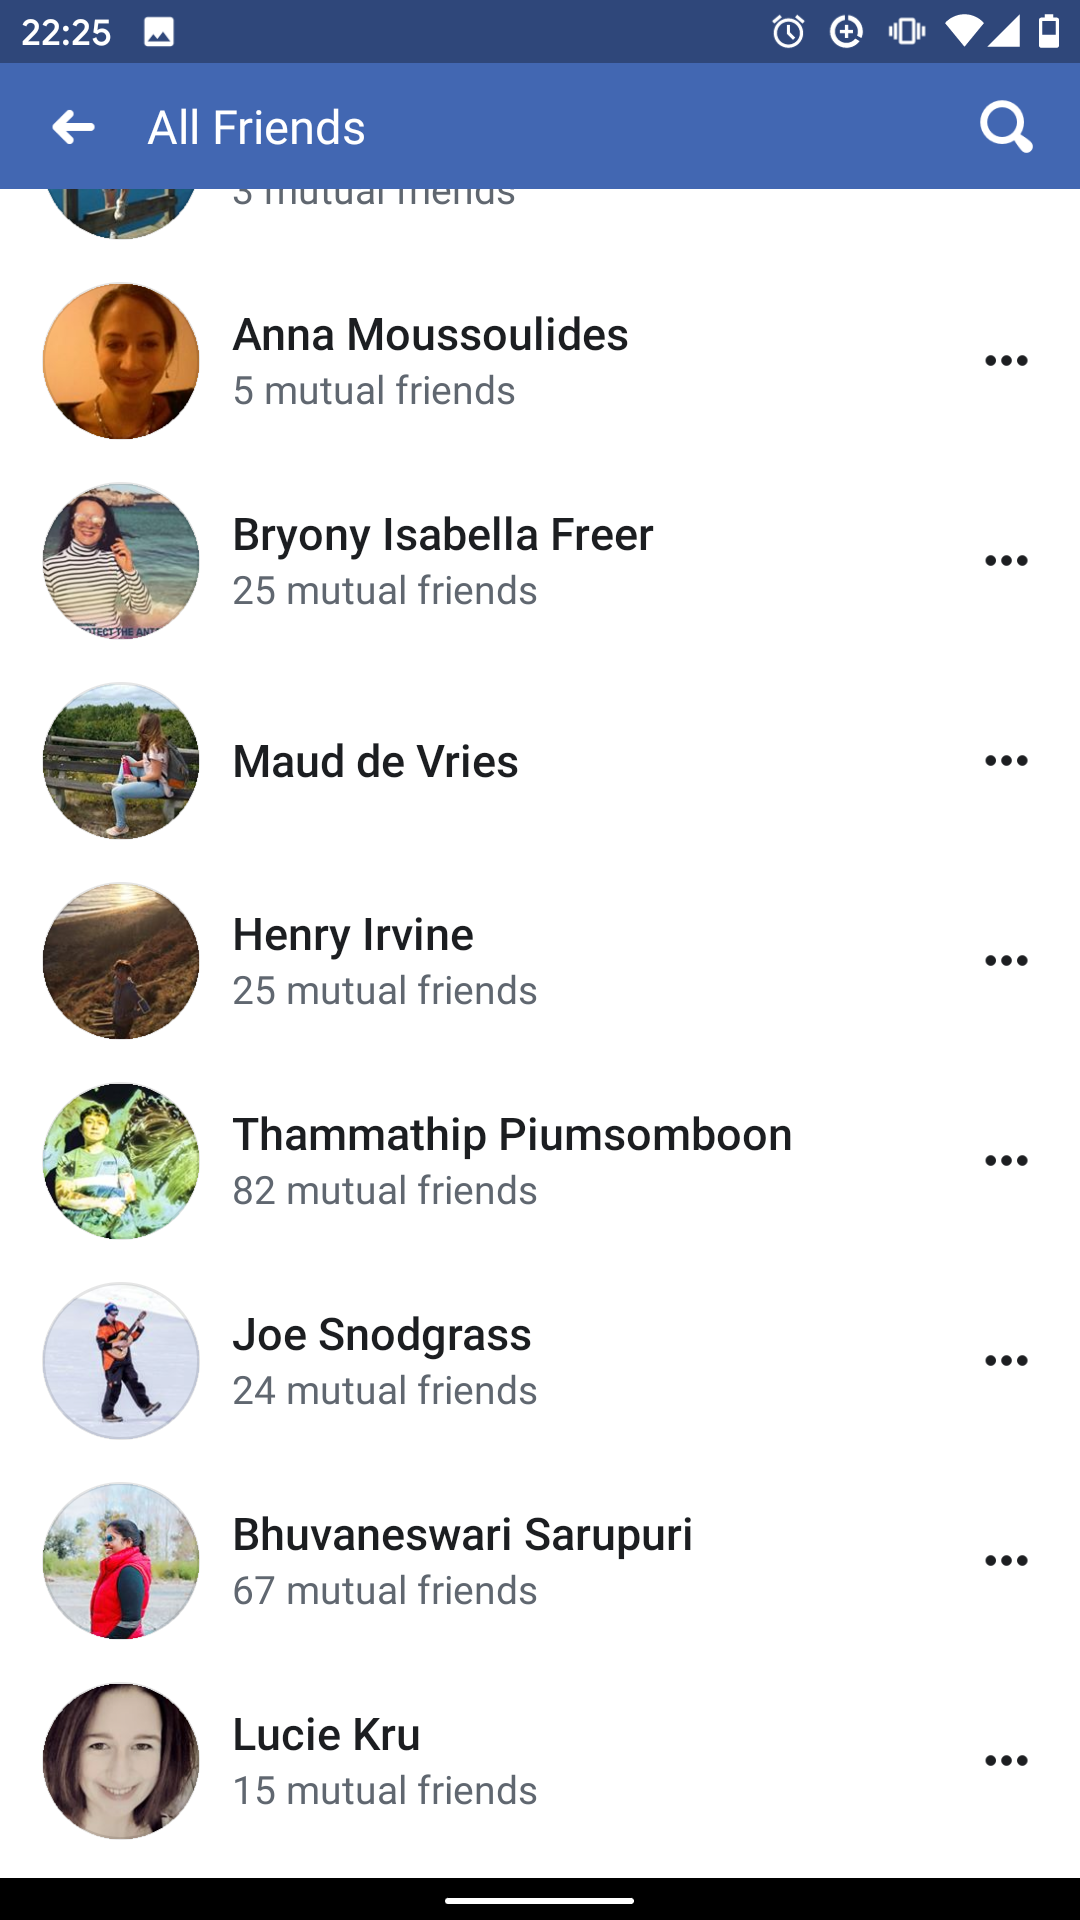
\includegraphics[width=0.8\linewidth]{images/41-visualising-mgia17/Screenshot_20190805-222553.}
    \caption{Changing Visual Fidelity across the social continuum}
    \label{fig:contacts:inspiration}
\end{figure}


The focus of this research is on how to represent a social network with hundreds of contacts in a wearable AR interface. If there are dozens of virtual tags in an AR view representing people, how can they be distinguished between each other? How will this scale to hundreds or thousands of people? The importance of this research is that it will allow users to view and interact with a large number of social network followers at different levels of privacy and social engagement.

Allowing users to view and interact with a large number of social contacts requires filtering and categorising information. One way to filter/categorise contacts could be to arrange them along a social continuum, depending on how close (in terms of social proximity) they are to the user. For example, grouping people into Intimate Family, Friends, Colleagues, and Strangers (see Table \ref{tbl:visual-fidelity-proximity}), or more categories. Contacts from these categories could then be shown as virtual avatars with different levels of visual fidelity and visual proximity, enabling the user to identify people in their social network quickly.

\begin{table}[h]
    \centering
    \caption{Using Visual Fidelity and Visual Proximity to Categorise Friends}
    \label{tbl:visual-fidelity-proximity}
    \begin{tabular}{|l|l|l|}
        \hline
        \textbf{Category} & \textbf{Visual Fidelity}    & \textbf{Visual Proximity}       \\ \hline
        Intimate          & 3D avatar                     & \textless1m, same space  \\ \hline
        Close friend      & 2D avatar                   & 1-5m, close              \\ \hline
        Acquaintance      & Bust image                    & 5-20m, nearby            \\ \hline
        Stranger          & Emoji                        & \textgreater20m, distant \\ \hline
    \end{tabular}
\end{table}


In terms of Visual Fidelity, the representations of people in each of these categories could be increasingly more realistic as the categories changed from Stranger to Intimate Family (see Figure \ref{fig:contacts:visual-fidelity-continuum}). For example, a user may see their spouse as a realistic 3D virtual human superimposed over the real world, but a distant acquaintance would be a simple 2D icon.

\begin{figure}[h]
    \centering
    \includegraphics[width=0.8\linewidth]{images/41-visualising-mgia17/writing-images-07.eps}
    \caption{Changing Visual Fidelity across the social continuum}
    \label{fig:contacts:visual-fidelity-continuum}
\end{figure}

In terms of proximity, previous studies have shown that the distance between people in social settings varies according to their level of intimacy \cite{Anslow2016}. This can be used to place the virtual representations of people in the real world around the user. The people that are Intimate family and Friends could be shown as visually closer to the user, while people who are Strangers would be shown further away (see Figure \ref{fig:contacts:proximic-circles}). This can be implemented as a body-centric virtual information space that travels with the user when they move.

The combination of using Visual Fidelity and Visual Proximity to categorise people from a user's social network could make it significantly easier for the viewer to pay attention to the people that they want to. For example, close Friends are represented as life-like virtual avatars near to the user, and so are easily distinguished from Strangers that are emoji icons further away.

\begin{figure}[h]
  \centering
  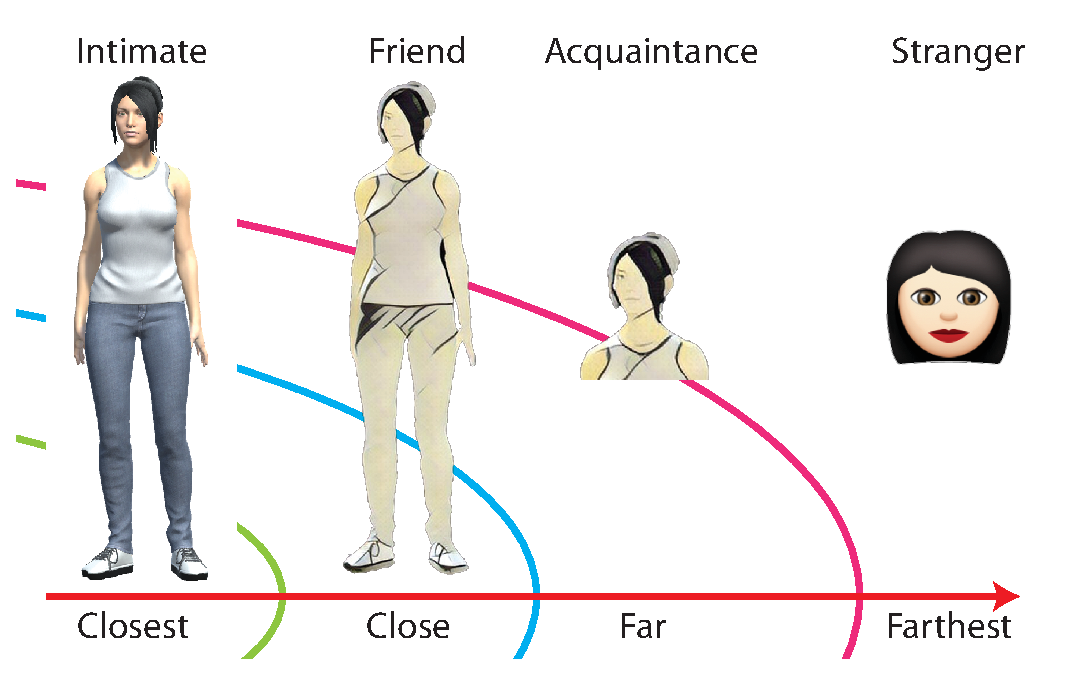
\includegraphics[width=0.8\linewidth]{images/41-visualising-mgia17/writing-images-11.eps}
  \caption{Visual Proxemic \& Visual Fidelity Filtering of Avatars}
    \label{fig:contacts:proximic-circles}
\end{figure}

% Other cues could be explored as well, such as placing people closer to the centre of the visual field who are more critical/active, using colour to distinguish which users are currently available, or providing spatial audio cues to guide a person's attention.


\subsection{Implementation}

Using the Social AR Continuum metaphor from the previous section, this work developed a prototype on the Microsoft HoloLens to represent a user's social contacts in an AR environment. The prototype was built using Unity3D\footnote{https://unity3d.com/} 5.6, HoloToolkit-Unity\footnote{https://github.com/Microsoft/HoloToolkit-Unity}, and 3D avatars from Morph3D\footnote{https://www.morph3d.com/}. Figure \ref{fig:contacts:overview} shows the AR view of the user's social network.

\begin{figure}[h]
  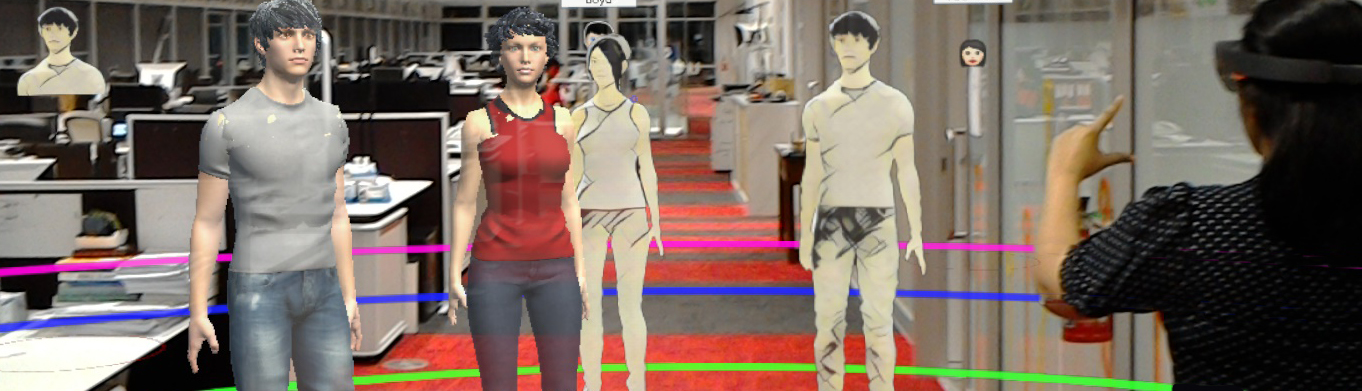
\includegraphics[width=\linewidth]{images/41-visualising-mgia17/20170618_031128_HoloLens_cropped.jpg}
  \caption{Representing social contacts in AR with different levels of proximity and visual fidelity}
  \label{fig:contacts:overview}
\end{figure}

Figure \ref{fig:contacts:system-diagram} shows an overview of the system components. The prototype uses the HoloLens Spatial Mapping feature to place virtual concentric circles (Circle Manager) on the ground around the user's initial position. On these circles, the social contacts are represented (Friend Manager) by either: a generic person silhouette, a 3D avatar, a 2D image, a bust image, or an emoji. The Scenario Manager controls the overall application, while the Friend Manager controls how friends are rendered. The Circle Manager controls the initial placement of the circles around the user. Spatial mapping is used to place circles and social contacts on the floor. Morph3D is used for rendering 3D avatars. 

\begin{figure}[h]
  \centering
  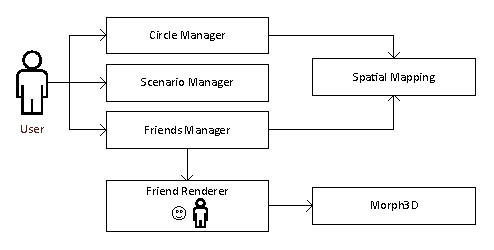
\includegraphics[width=0.8\linewidth]{images/41-visualising-mgia17/system-diagram.eps}
  \caption{System components}
    \label{fig:contacts:system-diagram}
\end{figure}

To arrange the social network, the user can use hand gestures (e.g., tap and drag) (Table \ref{tbl:contacts:gestures}) to move a virtual avatar closer or further away from the centre of the circles or change the social group the contact belongs to. The representation of the avatar automatically updates to match the selected social group. For instance, if the user selects a 3D avatar from the Intimate circle and moves it to the Friends circle, then their representation will turn into a bust image to reflect the target social group.

\begin{table}[h]
    \caption{Hand gestures used for interacting with social contacts through the HoloLens}
    \label{tbl:contacts:gestures}
    \centering
    \begin{tabular}{@{}lll@{}}
    \toprule
    Gesture      & Action                                       &  \\ \midrule
    Tap          & Select avatar                                &  \\
    Tap and hold & Move avatar between social proximity circles &  \\ \bottomrule
    \end{tabular}
\end{table}

\subsection{Focus Group Evaluation}

To evaluate the interface concept and collect feedback from potential users, this research conducted two focus group sessions with a total of 11 participants. The first group consisted of six post-graduate students working on AR/VR research. The second group was a mix of five professional visual graphics and user experience designers who have not worked on AR/VR before. Each session was divided into two activities: (1) user participatory design and (2) a usability test with the prototype. 

The focus group began with a discussion and brainstorming session on how to visualise social network contacts in an AR environment. The concept of social networking in AR was briefly introduced. A few challenges were observed, such as visual clutter, but no demonstration of the prototype system was given to avoid priming. This activity included three tasks: 

\begin{itemize}
    \item {Task 1: Imagine the future of social networks in AR. The participants were asked to draw or describe their vision of the future of how to represent social networks in AR. They then presented their ideas to the group and exchanged feedback.
    }
    
    \item {Task 2: Map social groups in terms of physical distance The participants were asked to order four different social groups (Intimate, Friend, Acquaintance, Stranger) in terms of physical distance from the user. Participants were given four silhouettes (Figure \ref{fig:contacts:silhouettes}) on paper that had one of the social groups written on the top and asked them to place them on an arrow that had four positions; closest, close, far and farthest.
\begin{figure}[ht]
    \centering
    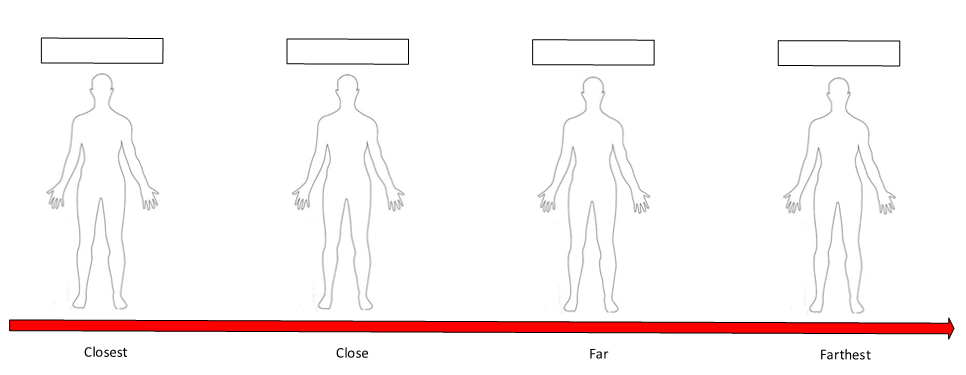
\includegraphics[width=\linewidth]{images/41-visualising-mgia17/silhouettes.PNG}
    \caption{Four placeholder for identifying the proximity of social relationships of a Friend, Strangers, Intimate, and Acquaintance}
    \label{fig:contacts:silhouettes}
\end{figure}
    }
    
    \item {Task 3: Map social groups in terms of visual fidelity. The participants were asked to match four different types of visual fidelity (3D avatar, 2D image, Bust image, Emoji) to four social groups (Intimate, Friend, Acquaintance, Stranger). This task included two sets of avatars, male and female.
\begin{figure}[ht]
    \centering
    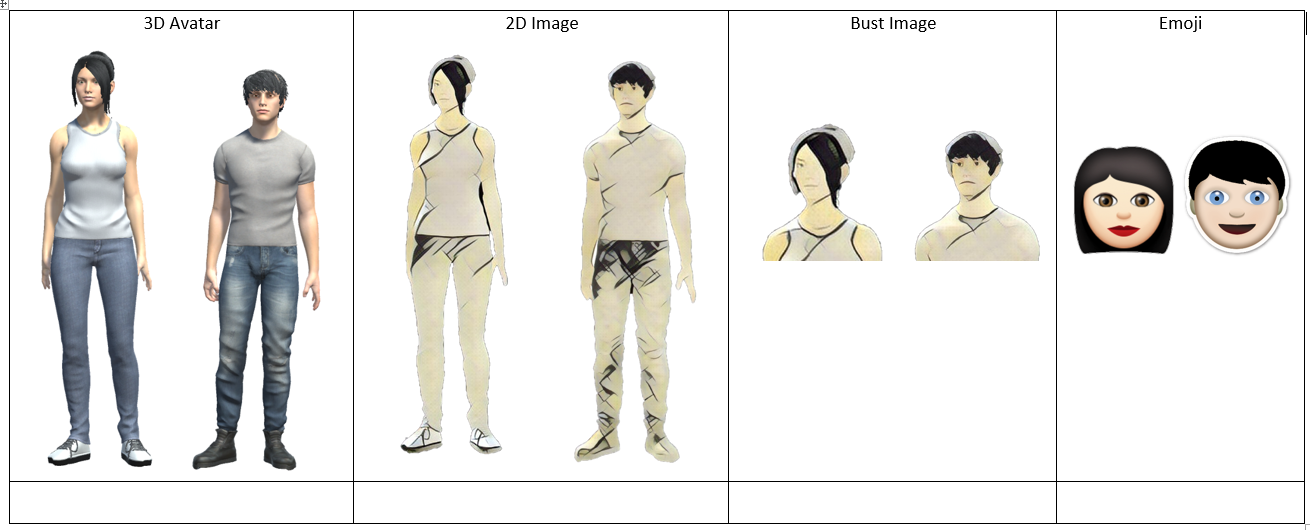
\includegraphics[width=\linewidth]{images/41-visualising-mgia17/avatars.PNG}
    \caption{Four placeholder for identifying the social relationships by an avatar representation of 3D avatar, 2D image, Bust image, Emoji}
    \label{fig:contacts:avatars}
\end{figure}    
    }
\end{itemize}

In the second session, the usability test, a demonstration was given of the prototype implementation, and the participants were asked for feedback on the following four conditions (see Figure \ref{fig:contacts:conditions}): 


\begin{itemize}
    \item{C1-Baseline (B): all avatars had the same visual representation (silhouette), and they were at the same distance away from the user.}
    
    \item{C2-Visual Proximity (P): the avatars were placed at different distances from the user based on their social intimacy (the Intimate group was the closest, then Friends, then Acquaintance, then Strangers). However, they were all a silhouette representation with the same Visual Fidelity.}
    
    \item{C3-Visual Fidelity (F): the avatars were placed at the same distance away from the viewer but had different visual representations based on their social group. The Intimate group was represented by an animated 3D avatar that moved and looked around. 2D static images represented friends, Acquaintances in 2D busts and Strangers were emojis.
    }
    \item{C4- Combined (C): both proximity and visual fidelity to filter social connections based on their social group.}

\end{itemize}

\begin{figure}[ht]
    \centering
    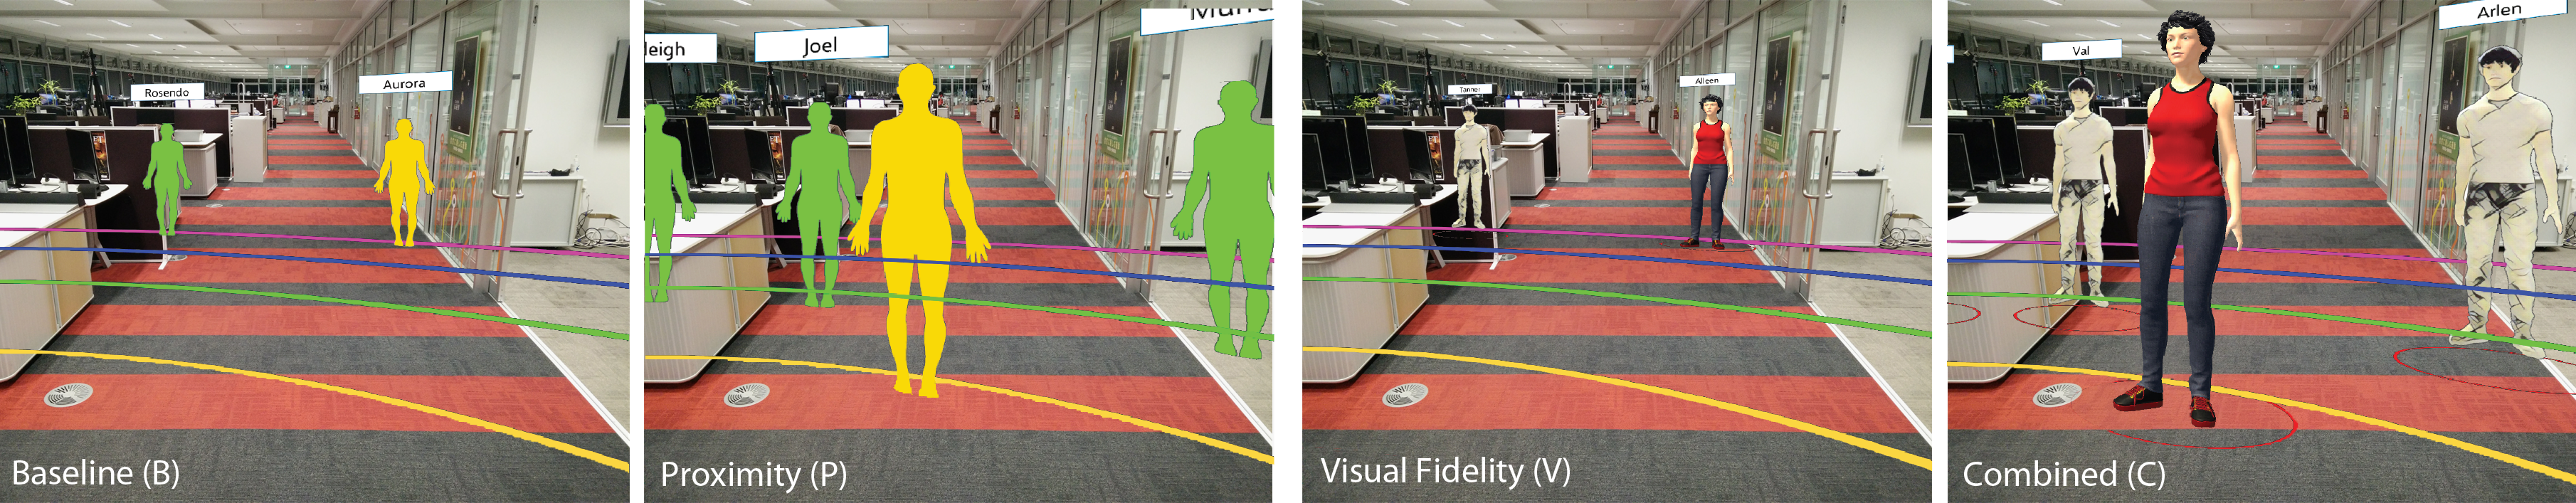
\includegraphics[width=\linewidth]{images/41-visualising-mgia17/conditions-transparent-background}
    \caption{Four conditions for representing social contacts as seen through the HoloLens. Baseline (B): fixed Visual Proximity and Visual Fidelity; Visual Proximity (P): variable Visual Proximity, but fixed Visual Fidelity; Visual Fidelity (V): same Visual Proximity, variable Visual Fidelity, and Combined (C): variable Visual Proximity and Visual Fidelity}
    \label{fig:contacts:conditions}
\end{figure}

Each participant tried the four conditions in random order, and for each condition, participants filled out a System Usability Scale (SUS) questionnaire \cite{brooke1996sus}. They also answered the following three personal questions, on a Likert scale from 1 to 7, where 1=\textit{Not very natural/easy} and 7=\textit{Very natural/easy}:

\begin{itemize}
    \item SQ1: How natural was the mapping of proximity to the social relationship?
    \item SQ2: How natural was the mapping of visual fidelity to the social relationship?
    \item SQ3: How easy was it to distinguish between the different avatar types?
\end{itemize}

\subsection{Results}

For this experiment, 11 participants were recruited, four female, aged between 16 and 41 years old, Median=29, SD=5.89. Most (85\%) used social networks (e.g., Facebook, Instagram, Snapchat) daily, and about 60\% reported using AR/VR headsets (e.g., HoloLens, HTC Vive) every month or more often. Only two people reported having no experience with AR/VR headsets before.

For \textit{Task 1}, when asked about how they would imagine representing social contacts in an AR platform, there were two main recurring themes, listed in order of popularity.

\textit{Theme 1 - Virtual Avatars}: Display virtual avatars representing friends around the users using spatial cues to distinguish them. The user can interact with other avatars to see their interests, posts or their location. The user can initiate a voice or video call with one of their contacts by interacting with the avatars.

% Mark: Did the people draw any pictures of their ideas? It would be good to include these as figures.

\textit{Theme 2 - Miniatures}: Display miniature avatars (spheres or bubbles) spread around the user environment, each bubble representing a friend. The locations of the bubbles could be determined by the social connection that the user has with that contact. Close friends could be placed near the user on a table surface while strangers are on the ground or further away. A user could pick up one of these bubbles and move them from one social group to another. The bubbles could follow the user when he moved to another place/room and re-arrange themselves according to the surrounding physical environment.

Other themes included seeing what others are seeing from their point of view, and highlighting who is online (coloured) or offline (greyed out) was also mentioned.
% Mark Billinghurst: Was there a difference between ideas suggests from HITLabNZ students and those people outside the lab?

% mark: [Do you have a list of all the 11 ideas? Maybe we can include that somehow]

% TODO (Gun): [Add a couple of sentences here (or in the discussion section) about how similar or different were the user's proposed design compared to our design (prototype system).]

For \textit{Task 2} (Figure \ref{fig:contacts:visual-fidelity}), participants were asked to order friend categories based on proximity (distance from the user). Most (90\%) participants ordered the categories as follows: Intimate, Friend, Acquaintance, Stranger on the scale from closest to furthest away from the user. This shows that users associated proximity to intimacy. Only one person chose: Intimate, Stranger, Friend, Acquaintance. 

\begin{figure}[ht]
    \centering
    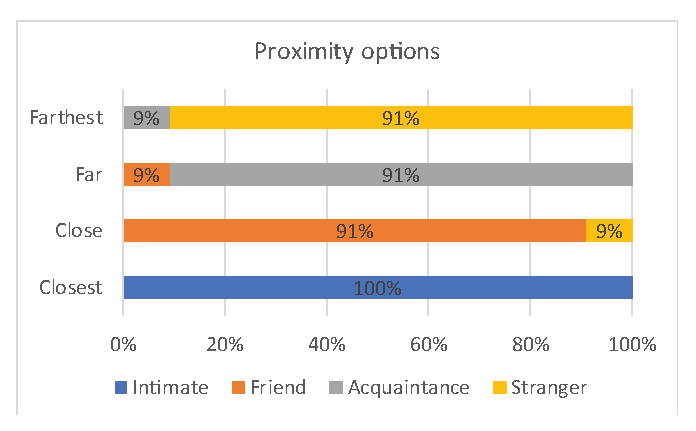
\includegraphics[width=0.8\linewidth]{images/41-visualising-mgia17/analysis-images-06.eps}
    \caption{Visual Fidelity categorisation for social contacts}
    \label{fig:contacts:visual-fidelity}
\end{figure}

For \textit{Task 3} (Figure \ref{fig:contacts:proximity}), participants were asked to categorise four types of visual fidelity. Most participants (73\%) associated 3D avatars with an Intimate relationship, 59\% marked the 2D image as a  Friend, 64\% associated the bust image for Acquaintances, while 45\% marked Emoji for Strangers. 14\% assigned 3D avatar with Stranger, a 2D image with Acquaintance, Bust images with Friend and Emoji with Intimate. 

% mark: In the discussion section, you might want to talk about the outliers
% mark: Maybe put this as a table?
% TODO (Gun): [Add here (or in the discussion section) how the results align with (or different from) our proposed design of the prototype system].
% mark: [It would be good to include comments from the users as to why they organised them in this way]

\begin{figure}[ht]
    \centering
    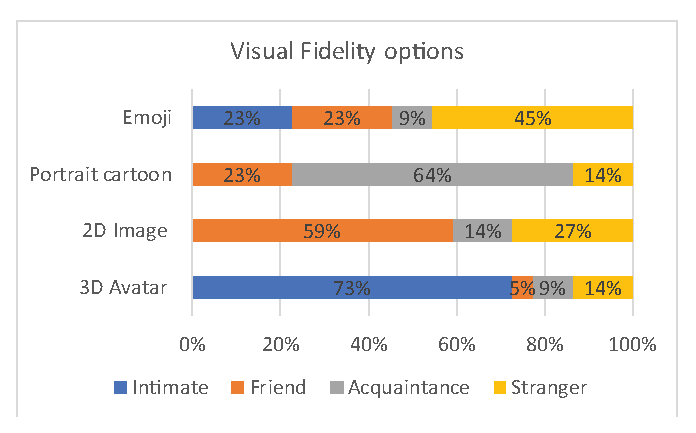
\includegraphics[width=0.8\linewidth]{images/41-visualising-mgia17/analysis-images-01.eps}
    \caption{Proximity categorisation for social contacts}
    \label{fig:contacts:proximity}
\end{figure}

The SUS scores (Figure \ref{fig:contacts:sus}) found that conditions C2-Proximity (69), C3-Visual Fidelity (69) and C4-Combined (72) were rated "Good" while C1-Baseline was "OK" (67). Data were tested for normality using Shapiro-Wilk test and found to be normally distributed ($p=0.83, 0.779, 0.292, 0.188$ for C1, C2, C3 and C4 respectively). To see if this difference was statistically significant, an aligned rank transform was run on the SUS results in order to run a 2-way repeated measure ANOVA analysis with two factors Proximity and Visual Fidelity. No significant differences ($F(1, 10)=1.414,p=0.262$) were found in terms of SUS between Proximity and Visual Fidelity. 

\begin{figure}[ht]
    \centering
    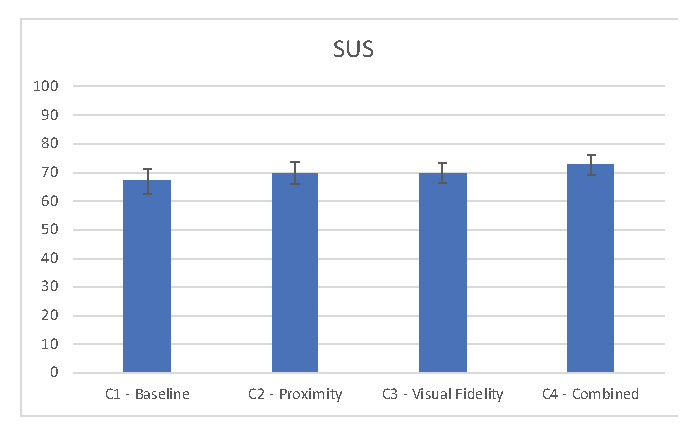
\includegraphics[width=0.8\linewidth]{images/41-visualising-mgia17/analysis-images-02.eps}
    \caption{The System Usability Score. Whiskers indicate standard error.}
    \label{fig:contacts:sus}
\end{figure}
% TODO (Gun): In the figure caption, you should mention what does the whiskers (error bars) represent. BTW, based on the error bars seems you might have had significant results? Any inferential statistics to report here? I would suggest running Aligned Rank Transform Repeated-measure two-way ANOVA. 
% mark: You should label them B, P, F and C

The subjective questionnaire (Figure \ref{fig:contacts:sq2}) shows an increase in how natural people felt the mapping to proximity (SQ1) was in the Proximity condition. A Friedman test was run and found that there was a statistically significant difference in rating the four conditions, ($\chi^2(2)=18.402,p<0.001$). Post hoc analyses with Wilcoxon signed-rank tests were conducted with a Bonferroni correction applied, resulting in a significance level set at ($alpha=0.008$). There was a significant difference between conditions C4-Combined and C1-Baseline ($Z=-2.687, p=0.007$). However, there were no statistically significant differences between the other conditions.

\begin{figure}[ht]
    \centering
    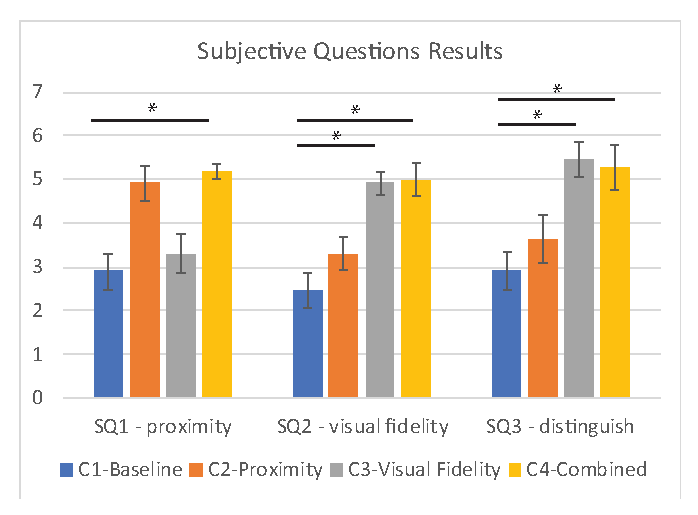
\includegraphics[width=0.8\linewidth]{images/41-visualising-mgia17/analysis-images-05.eps}
    \caption{Subjective question results by condition by question. Whiskers indicate standard error. *=statistically significant difference}
    \label{fig:contacts:sq2}
\end{figure}

Similarly, there was an increase in how natural people felt the mapping to visual fidelity (SQ2) was in the Visual Fidelity condition. Running a Friedman test found that there was a statistically significant difference in rating the four conditions, ($\chi^2(2)=21.194,p<0.001$). Post hoc analyses with Wilcoxon signed-rank tests were conducted with a Bonferroni correction applied, resulting in a significance level set at $alpha=0.008$. There were significant differences between conditions C3-Visual Fidelity and C1-Baseline ($Z=-2.825, p=0.005$) and between conditions C4-Combined and C1-Baseline ($Z=-2.820, p=0.005$). However, there were no statistically significant differences between the other conditions.

As for the (SQ3), people felt it was easier to distinguish between different avatars in both the Visual Fidelity and Combined conditions. Running a Friedman test found that there was a statistically significant difference in rating the four conditions, ($\chi^2(2)=20.967,p<0.001$). Post hoc analyses with Wilcoxon signed-rank tests were conducted with a Bonferroni correction applied, resulting in a significance level set at $alpha=0.008$. There were significant differences between conditions C3-Visual Fidelity and C1-Baseline ($Z=-2.816, p=0.005$) and between conditions C4-Combined and C1-Baseline ($Z=-2.829, p=0.005$). However, there were no statistically significant differences between the other conditions.


For ranking the conditions (Figure \ref{fig:contacts:ranking}), participants ranked the four conditions from 4 to 1, where four was the most preferred and one the least preferred. Results show that participants preferred conditions C3-Visual Fidelity and C4-Combined over C2-Proximity and C1-Baseline. A Friedman test found that there was a statistically significant difference in ranking the four conditions ($\chi^2(2)=15.222,p=0.002$). Post hoc analyses with Wilcoxon signed-rank tests were conducted with a Bonferroni correction applied, resulting in a significance level set at $alpha=0.008$. There was a significant difference between C3-Visual Fidelity and C1-Baseline ($Z=-3.035, p=0.002$). However, there were no statistically significant differences between the other conditions.

\begin{figure}[ht]
    \centering
    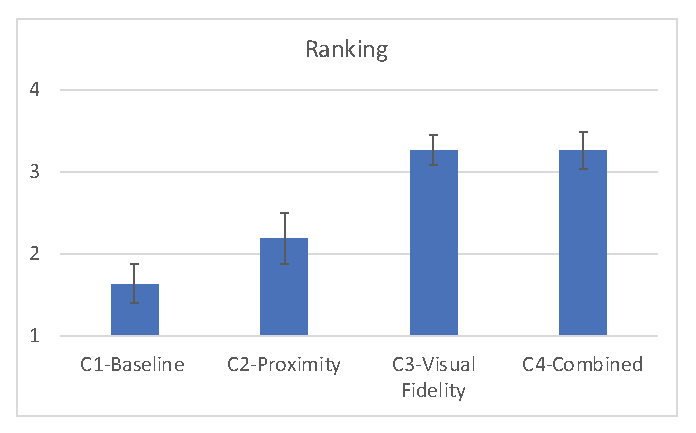
\includegraphics[width=0.8\linewidth]{images/41-visualising-mgia17/analysis-images-04.eps}
    \caption{Ranking (4=highest, 1=lowest). Whiskers indicate standard error.}
    \label{fig:contacts:ranking}
\end{figure}

\subsection{Discussion}

The user study results found that subjects preferred having a filter to represent their social contacts rather than no filter (i.e., Baseline condition). Based on the ranking results, the most preferred filters are the Visual Fidelity and Combined filters, followed by the Proximity filter.
% TODO (Gun) : [Discuss how this is similar to our proposed design or what is the difference? How this would affect further development/design of the social AR interface?]
The subjective questions revealed that each condition was representing the natural mapping/filter of the user's social contacts (i.e., "SQ1-how natural the proximity" scored high in "P" and so on). Participants felt that the Visual Fidelity condition (V) was the easiest for distinguishing avatars.

In terms of the strengths and weaknesses of each condition, participants did not like the Baseline condition because they could not easily distinguish the avatars. For example, one participant said, "\textit{I cannot distinguish avatar so well, I do not want to look around at everyone at the same distance}". This confirms our original predictions regarding the placing of social contacts.

With the Proximity condition, participants reported positive feedback and an increase in avatar presence, but they were not able to adequately distinguish users from each other.  One user said "\textit{I feel more spatial presence}", but another said "\textit{I need to look around more to see what is where.}"

In the Visual Fidelity condition, participants reported that it was easy to distinguish between contacts, but the interface could be improved. One user said "\textit{This one felt more comfortable with people at a distance and was easy to tell people apart}", while another user said, "\textit{Take more visual space for people whom I do not want to interact with.}"

For the Combined condition, participants reported it was the best because they felt that it was easier to distinguish between avatars. One user said "\textit{More info is available (fidelity + distance)..}".
However, some participants did not like it when the avatars were too close and recommended increasing the minimum distance between the user and the closest circle.

The limitations of this work include that the avatars are not a true representation of the participants' social contacts. This study assumes a predefined set of social contacts mixed between male and female and different outfits. This system assumes four levels of social relationships: 1) intimate, 2) friend, 3) acquaintance and 4) stranger. Users may have fewer or more levels of social contacts. 

Overall, the results confirmed our hypothesis that users would prefer to have their social contacts filtered out based on their relationship to them. The question was which filter (Proximity or Visual Fidelity) is best for each condition. Users seem to prefer either visual fidelity or a combination of visual fidelity and proximity. This may remain a user preference. 

% Tobias: You do not discuss shortcomings/limitations of the study (e.g. internal and external validity). This should all come into the discussion sections, which is missing, as stated before.

\subsection{Conclusions}

This section investigated different visualisation options for representing social contacts in a wearable AR interface. Two focus groups were conducted to get feedback from potential users about how they would want to organise social contacts in an AR interface. Participants identified visual representation and spatial cues as common ways to do this. This matched the interface metaphor used to develop a working prototype.

The user study measured the usability and user preference of four conditions in a prototype AR interface on a HoloLens display: 1) Baseline, 2) Proximity, 3) Visual Fidelity and 4) Combined. Participants indicated that it was useful to have some different visual fidelity representations of their AR social contacts and that combined use of visual fidelity and proximity was also useful. These conditions highlight the dimension of representing social contacts on the Social AR Continuum. The next section looks into the dimension of placing social contacts. 

% In the future, we plan to explore and further develop different visual fidelity representations of social contacts (e.g., displaying avatars as miniatures on a nearby surface). We will also investigate different ways to interact with other users in social networks who are either physically collocated or remote.
